%% THESIS — the school format, taken unchanged from the pre-thesis report
%% (docs/Pre-thesis/Latex/main_docx.tex). Only the title page wording, the "Thesis additions" block
%% and the chapter list differ. Build: latexmk -pdf main.tex (in this folder).
\documentclass[12pt, twoside]{report}
% \documentclass[12pt, twoside, draft]{report} - Xuất file ko hình ảnh = xoá %

%% ── Encoding & Language ──────────────────────────────────────────────────────
\usepackage[T1]{fontenc}
\usepackage[utf8]{inputenc}
\usepackage[main=english]{babel}

%% ── Math ─────────────────────────────────────────────────────────────────────
\usepackage{amsmath}
\usepackage{amssymb}

%% ── Symbols ──────────────────────────────────────────────────────────────────
\usepackage{pifont}
\newcommand{\cmark}{\ding{51}}%
\newcommand{\xmark}{\ding{55}}%

%% ── Tables ───────────────────────────────────────────────────────────────────
\usepackage{multirow}
\usepackage{booktabs}
%% longtable: allows tables to break across pages
\usepackage{longtable}
%% tabularx: for auto-width columns
\usepackage{tabularx}

%% ── Graphics ─────────────────────────────────────────────────────────────────
\usepackage{graphicx}
\usepackage{tikz}
\usetikzlibrary{calc}
\usepackage{float}   % provides [H] float specifier (place figure HERE exactly)

%% ── Page Layout (identical to main.tex) ─────────────────────────────────────
\usepackage[a4paper, top=2.5cm, bottom=2cm, left=3cm, right=2cm, bindingoffset=5mm]{geometry}
\usepackage{fancyhdr}
\usepackage{titlesec}

%% ── Paragraph indentation & Line Spacing ───────────────────────────────────────
%% indentfirst: indent the FIRST paragraph after section headings (matches Word style)
\usepackage{indentfirst}
\usepackage{setspace}            % for \onehalfspacing (matches docx 1.5 line spacing)
\usepackage{enumitem}            % for clean reference list without bullets
\setlength{\parindent}{1.25cm}   % Word default first-line indent
\setlength{\parskip}{4pt}        % small inter-paragraph spacing
\raggedbottom                    % prevent vertical stretch that creates page gaps

%% ── Algorithms & Listings ────────────────────────────────────────────────────
\usepackage{algorithm}
\usepackage{algpseudocode}
\usepackage{url}
\usepackage{listings}
\usepackage{xcolor}

%% Customize listings style (same as main.tex)
\lstdefinestyle{mystyle}{
	basicstyle=\ttfamily\footnotesize,
	breakatwhitespace=false,
	breaklines=true,
	captionpos=b,
	frame=single,
	keepspaces=true,
	numbers=left,
	numbersep=5pt,
	numberstyle=\tiny\color{black},
	showstringspaces=false,
}
\lstset{style=mystyle}
\lstdefinelanguage{JavaScript}{
	morekeywords=[1]{break, continue, delete, else, for, function, if, in,
	new, return, this, typeof, var, void, while, with},
	morekeywords=[2]{false, null, true, boolean, number, undefined,
	Array, Boolean, Date, Math, Number, String, Object},
	morekeywords=[3]{eval, parseInt, parseFloat, escape, unescape},
	sensitive,
	morekeywords=[4]{await, async, case, catch, class, const, default, do,
		enum, export, extends, finally, from, implements, import, instanceof,
	let, static, super, switch, throw, try},
	morecomment=[s]{/*}{*/},
	morecomment=[l]//,
	morecomment=[s]{/**}{*/},
	morestring=[b]',
	morestring=[b]",
	keywordstyle={[1]\color{teal}\bfseries},
	keywordstyle={[2]\color{red}\bfseries},
	keywordstyle={[3]\color{violet}\bfseries},
	keywordstyle={[4]\color{blue}\bfseries},
	commentstyle=\color{gray}\ttfamily,
	stringstyle=\color{orange}\ttfamily,
}

%% ── Chapter title format (identical to main.tex) ────────────────────────────
\titleformat{\chapter}[display]
  {\Huge\bfseries\centering}{\chaptername~\thechapter}
  {0pt}
  {\Huge}
\titlespacing*{\chapter}
  {0pt}
  {*0}
  {1em}

%% ── Appendix labeling (identical to main.tex) ───────────────────────────────
\makeatletter
\newcommand\AppendixName{Appendix}
\let\oldappendix\appendix
\renewcommand{\appendix}{%
  \oldappendix
  \renewcommand{\chaptername}{\AppendixName}
  \renewcommand{\thechapter}{\@Alph\c@chapter}}
\makeatother

%% ── Captions & TOC names ─────────────────────────────────────────────────────
\addto\captionsenglish{\renewcommand*\contentsname{Table of Contents}}
\addto{\extrasenglish}{\renewcommand{\bibname}{References}}
\renewcommand\lstlistlistingname{List of Listings}

%% ── Graphics path ────────────────────────────────────────────────────────────
\graphicspath{{images/}}

%% ── Hyperlinks (optional but useful) ────────────────────────────────────────
\usepackage[hidelinks]{hyperref}

%% ── Remove chapter prefix from figure/table numbers in LoF/LoT ──────────────
%% 1) Make the counter sequential across ALL chapters (no reset per chapter)
\usepackage{chngcntr}
\counterwithout{figure}{chapter}
\counterwithout{table}{chapter}
%% 2) Display as plain arabic (no "3." prefix)
\renewcommand{\thefigure}{\arabic{figure}}
\renewcommand{\thetable}{\arabic{table}}
%% 3) Format LoF/LoT entries as "Figure N." and "Table N." using tocloft
\usepackage{tocloft}
\renewcommand{\cftfigpresnum}{Figure~}
\renewcommand{\cftfigaftersnum}{.}
\setlength{\cftfignumwidth}{5.5em}
\renewcommand{\cfttabpresnum}{Table~}
\renewcommand{\cfttabaftersnum}{.}
\setlength{\cfttabnumwidth}{5em}

%% ─────────────────────────────────────────────────────────────────────────────
%% ── Thesis additions ─────────────────────────────────────────────────────────
%% Every result number is a macro written by `npm run report -w @breadit/eval`, never a typed number.
%% Tables: \input{\resultsdir/tables/<id>.tex}. Figures: pgfplots reading the CSVs of \resultsdir.
\usepackage{pgfplots}
\pgfplotsset{compat=1.18}
\newcommand{\resultsdir}{../results/p7-report}
\input{\resultsdir/results-macros.tex}
%% Citation by key: \refcite{<key>} prints [n], the number of the item with \label{ref:<key>} in chapters/references.tex.
\newcommand{\refcite}[1]{[\ref{ref:#1}]}
%% Diagram by name: \thesisdiagram{<name>}{<width>} shows images/<name>.pdf if it exists, else images/<name>.png,
%% else a framed placeholder. The author only saves the image (see diagrams.md); no .tex edit. The image is never taller than 80% of the text,
%% unless the optional first argument gives another maximum height (the ERD: \thesisdiagram[0.87\textheight]{fig4-11-erd}{\textwidth}).
\newcommand{\thesisdiagram}[3][0.8\textheight]{%
  \IfFileExists{images/#2.pdf}{\includegraphics[width=#3,height=#1,keepaspectratio]{#2.pdf}}{%
  \IfFileExists{images/#2.png}{\includegraphics[width=#3,height=#1,keepaspectratio]{#2.png}}{%
  \fbox{\parbox[c][5cm][c]{0.9\textwidth}{\centering Figure to be drawn: \texttt{images/#2.pdf}}}}}}

%% The title registered with the school. Change it here only: the title page uses it twice.
\newcommand{\thesistitle}{Breadit: A real-time hybrid social networking platform with social-graph-aware personalized feed ranking}

\begin{document}
\onehalfspacing                  % match docx 1.5 line spacing
\pagenumbering{roman}

\newgeometry{top=2.5cm, bottom=2.5cm, left=2.5cm, right=2.5cm}

%% ── TITLE PAGE ───────────────────────────────────────────────────────────────
\begin{titlepage}

	\begin{tikzpicture}[remember picture,overlay,inner sep=0,outer sep=0]
     \draw[blue!70!black,line width=4pt] ([xshift=-1.5cm,yshift=-2cm]current page.north east) coordinate (A)--([xshift=1.5cm,yshift=-2cm]current page.north west) coordinate(B)--([xshift=1.5cm,yshift=2cm]current page.south west) coordinate (C)--([xshift=-1.5cm,yshift=2cm]current page.south east) coordinate(D)--cycle;

     \draw ([yshift=0.5cm,xshift=-0.5cm]A)-- ([yshift=0.5cm,xshift=0.5cm]B)--
     ([yshift=-0.5cm,xshift=0.5cm]B) --([yshift=-0.5cm,xshift=-0.5cm]B)--([yshift=0.5cm,xshift=-0.5cm]C)--([yshift=0.5cm,xshift=0.5cm]C)--([yshift=-0.5cm,xshift=0.5cm]C)-- ([yshift=-0.5cm,xshift=-0.5cm]D)--([yshift=0.5cm,xshift=-0.5cm]D)--([yshift=0.5cm,xshift=0.5cm]D)--([yshift=-0.5cm,xshift=0.5cm]A)--([yshift=-0.5cm,xshift=-0.5cm]A)--([yshift=0.5cm,xshift=-0.5cm]A);

     \draw ([yshift=-0.3cm,xshift=0.3cm]A)-- ([yshift=-0.3cm,xshift=-0.3cm]B)--
     ([yshift=0.3cm,xshift=-0.3cm]B) --([yshift=0.3cm,xshift=0.3cm]B)--([yshift=-0.3cm,xshift=0.3cm]C)--([yshift=-0.3cm,xshift=-0.3cm]C)--([yshift=0.3cm,xshift=-0.3cm]C)-- ([yshift=0.3cm,xshift=0.5cm]D)--([yshift=-0.3cm,xshift=0.3cm]D)--([yshift=-0.3cm,xshift=-0.3cm]D)--([yshift=0.3cm,xshift=-0.3cm]A)--([yshift=0.3cm,xshift=0.3cm]A)--([yshift=-0.3cm,xshift=0.3cm]A);

   \end{tikzpicture}

	\centering
	\textbf{VIETNAM NATIONAL UNIVERSITY OF HO CHI MINH CITY}\par
	\textbf{THE INTERNATIONAL UNIVERSITY}\par
	\textbf{SCHOOL OF COMPUTER SCIENCE AND ENGINEERING}\par

	\vspace{1.5cm}
	
\includegraphics[width=0.3\textwidth]{images/IU.png}

	\vspace{1.5cm}
	\textbf{\large \thesistitle}

	\vspace{1.5cm}
	By \par \textbf{Cao Ngoc Anh Tuan -- ITCSIU21244}

	\vspace{4.5cm}
	\textit{A thesis submitted to the School of Computer Science and Engineering \\
		in partial fulfillment of the requirements for the degree of \\
		Bachelor of Computer Science}

	\vspace{2cm}
	\text{Ho Chi Minh City, Vietnam} \par 2026

	\newpage

	%% Signature page
	\centering
	\textbf{\large \thesistitle}\par
	\vspace{4cm}

	\hspace{7cm}
	\makebox[7cm][l]{\text{APPROVED BY:}}
	\par
	\vspace{2cm}

	\hspace{7cm}
	\makebox[7cm][l]{\underline{\hspace{7cm}}}
	\par \hspace{7cm}
	\makebox[7cm][l]{\textit{MSc. Nguyen Trung Nghia}}
	\par
	\vspace{2cm}

	\hspace{7cm}
	\makebox[7cm][l]{\underline{\hspace{7cm}}}
	\par \hspace{7cm}
	\makebox[7cm][l]{\textit{Committee name here}}
	\par
	\vspace{2cm}

	\hspace{7cm}
	\makebox[7cm][l]{\underline{\hspace{7cm}}}
	\par \hspace{7cm}
	\makebox[7cm][l]{\textit{Committee name here}}
	\par
	\vspace{2cm}

	\hspace{7cm}
	\makebox[7cm][l]{\underline{\hspace{7cm}}}
	\par \hspace{7cm}
	\makebox[7cm][l]{\textit{Committee name here}}
	\par
	\vspace{2cm}

	\hspace{7cm}
	\makebox[7cm][l]{\underline{\hspace{7cm}}}
	\par \hspace{7cm}
	\makebox[7cm][l]{\textit{Committee name here}}
	\par
	\vspace{0.75cm}

	\hspace{7cm}
	\makebox[7cm][r]{\text{THESIS COMMITTEE}}
	\par
	\thispagestyle{empty}
\end{titlepage}
\restoregeometry

%% ── ACKNOWLEDGEMENTS ─────────────────────────────────────────────────────────
\chapter*{Acknowledgements}
\addcontentsline{toc}{chapter}{Acknowledgements}
% Acknowledgements. Draft: drafts/(none)
% Numbers: macros only (\resultsdir/results-macros.tex), never typed by hand.

\thispagestyle{empty}

%% ── LISTS OF CONTENTS ────────────────────────────────────────────────────────
\newpage
\tableofcontents
\newpage
\listoftables
\addcontentsline{toc}{chapter}{List of Tables}
\newpage
\listoffigures
\addcontentsline{toc}{chapter}{List of Figures}
\newpage

%% ── ABSTRACT ─────────────────────────────────────────────────────────────────
\chapter*{Abstract}
\addcontentsline{toc}{chapter}{Abstract}
% Abstract. Draft: drafts/00-abstract.md
% Numbers: macros only (\resultsdir/results-macros.tex), never typed by hand.


%% ── CHAPTERS ─────────────────────────────────────────────────────────────────
%% Nine chapters, about 95 pages (drafts/Report Architecture.md). Each chapter has its Markdown draft in drafts/.
\chapter{INTRODUCTION}
\pagenumbering{arabic}
\setcounter{page}{1}
% Chapter 1. Introduction. Draft: drafts/01-introduction.md
% Numbers: macros only (\resultsdir/results-macros.tex), never typed by hand.


\chapter{LITERATURE REVIEW}
% Chapter 2. Literature Review. Draft: drafts/02-literature-review.md
% Numbers: macros only (\resultsdir/results-macros.tex), never typed by hand.


\chapter{METHODOLOGY}
% Chapter 3. Methodology. Draft: drafts/03-methodology.md
% Numbers: macros only (\resultsdir/results-macros.tex), never typed by hand.


\chapter{SYSTEM ANALYSIS AND DESIGN}
% Chapter 4. System Analysis and Design. Draft: drafts/04-system-analysis-and-design.md
% Numbers: macros only (\resultsdir/results-macros.tex), never typed by hand.


\chapter{IMPLEMENTATION}
% Chapter 4. Implementation. Draft: drafts/04-implementation.md
% Numbers: macros only (\resultsdir/results-macros.tex), never typed by hand.


\chapter{EXPERIMENTS AND RESULTS}
% Chapter 5. Experiments and Results. Draft: drafts/05-experiments-and-results.md
% Numbers: macros only (\resultsdir/results-macros.tex), never typed by hand.


\chapter{DISCUSSION}
% Chapter 6. Discussion. Draft: drafts/06-discussion.md
% Numbers: macros only (\resultsdir/results-macros.tex), never typed by hand.


\chapter{TEST CASES AND DEMONSTRATION}
% Chapter 8. Test Cases and Demonstration. Draft: drafts/08-test-cases-and-demonstration.md
% Numbers: macros only (\resultsdir/results-macros.tex), never typed by hand.


\chapter{CONCLUSION \& FUTURE WORKS}
% Chapter 9. Conclusion and Future Works. Draft: drafts/09-conclusion-and-future-works.md
% Numbers: macros only (\resultsdir/results-macros.tex), never typed by hand.


%% ── REFERENCES ───────────────────────────────────────────────────────────────
\chapter*{References}
\addcontentsline{toc}{chapter}{References}
% References: the numbered list of the school format (same as the pre-thesis report).
% Cite only references marked "verified" in the super-plan §10. Uncomment the list with the first item:
% \begin{enumerate}[leftmargin=*, label=\arabic*., itemsep=0.8em]
%   \item Holm, S. (1979). A simple sequentially rejective multiple test procedure. \textit{Scandinavian Journal of Statistics}, 6(2).
% \end{enumerate}


%% ── APPENDIX ─────────────────────────────────────────────────────────────────
% \appendix switches counter to A, B, C... but also auto-prefixes "Appendix A"
% Using \chapter*{} suppresses that prefix so only "APPENDIX" appears
\appendix
\chapter*{APPENDIX}
\addcontentsline{toc}{chapter}{APPENDIX}
% Appendix. Draft: drafts/10-appendix.md
% Numbers: macros only (\resultsdir/results-macros.tex), never typed by hand.


\end{document}
